\documentclass[11pt]{article}
\usepackage[letterpaper,margin=1in]{geometry}
\usepackage[T1]{fontenc}
\usepackage{lmodern,amsmath,amssymb,booktabs,microtype}
\usepackage{graphicx}
\graphicspath{{routing_note/}{./}}
\begin{document}
\begin{center}
{\LARGE One-stop routing with a changing distance cutoff}\\[6pt]
Jonathan R. Landers
\end{center}

Suppose a planner has fixed two terminals and a list of possible transfer
stops. The planner wants the shortest route through exactly one stop and is
exploring different requirements for the minimum separation of the three
locations. A single query takes one pass over the list. Repeating that pass
for each cutoff discards a useful piece of information: once a route fails,
raising the cutoff can never bring it back. We use that ordering to answer
each subsequent query by binary search.

\paragraph{The route as a triangle.}
Let $A,B\in\mathbb R^2$ be the terminals and $V_1,\ldots,V_n$ the candidate
stops. Write $d$ for Euclidean distance. Each route has two numbers,
\[
 q_i=\min\{d(A,V_i),d(V_i,B),d(A,B)\},\qquad
 L_i=d(A,V_i)+d(V_i,B).
\]
The two traveled legs determine the cost $L_i$. All three pairs must meet the
separation requirement, so $q_i$ includes the terminal separation. At cutoff
$k>0$ the query asks for the smallest pair $(L_i,i)$ in lexicographic order
among stops with $q_i\ge k$. The second coordinate breaks ties by input order.
An empty feasible set yields no route. Collinear stops are permitted.

The triangle companion derives a shape threshold from the ratio $S$ of shortest
to longest side. At triangle diameter $D_i$, the unnormalized threshold is
precisely $D_i S_i=q_i$ whenever $D_i>0$. Computing $q_i$ directly also
handles coincident locations. To see the scaling law, multiply every coordinate
by $\lambda>0$. Each side, and hence its minimum and maximum, is multiplied by
$\lambda$. Thus $S_i$ stays fixed and the least admissible diameter is
$k/S_i$ for $S_i>0$. In the routing problem the coordinates stay fixed and the
cutoff varies, so the same inequality reads $k\le q_i$. It holds pointwise
for any placement of stops.


\paragraph{A change of stop.}
Take $A=(0,0)$ and $B=(4,0)$. A stop at $(1,0)$ yields length $4$ and
threshold $1$. A stop at $(2,1)$ yields length $2\sqrt5$ and threshold
$\sqrt5$. The shorter route wins through $k=1$. For $1<k\le\sqrt5$ the
detour wins, and above $\sqrt5$ both fail. The table records that change of
winner during construction, before any query is known.


\begin{center}
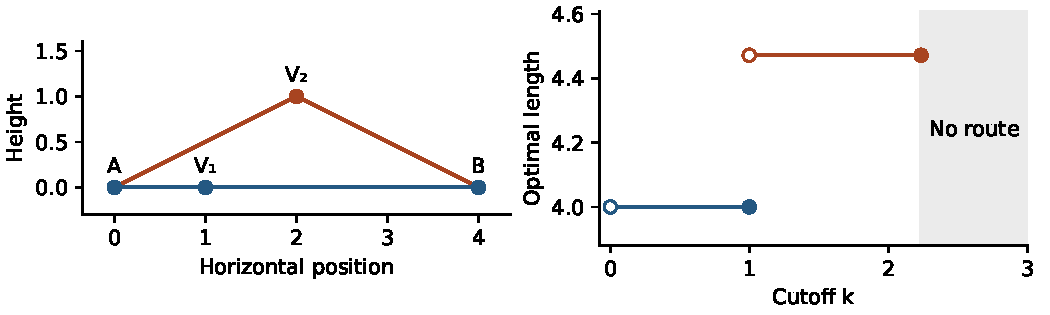
\includegraphics[width=.94\linewidth]{route_geometry.pdf}\\
\small Figure 1. Both candidate paths and the resulting optimum. Filled endpoints
include equality. Grey denotes infeasibility.
\end{center}
\newpage
\paragraph{Index theorem.}
\textit{With fixed terminals and stops, $O(n\log n)$ preprocessing and $O(n)$
storage suffice to return an optimal stop and its route length, or report
infeasibility, in $O(\log(n+1))$ time per query for $n\ge1$.}

\paragraph{Construction and proof.}
Sort the indices into an order $\pi$ with
$q_{\pi(1)}\ge\cdots\ge q_{\pi(n)}$. At position $j$ store the index $w_j$
that minimizes $(L_i,i)$ over the first $j$ positions. Start with
$w_1=\pi(1)$. To extend the table, keep the better of $w_{j-1}$ and $\pi(j)$.
Induction gives the stated minimum at every position.

For a query, binary search for the last position $j$ with $q_{\pi(j)}\ge k$.
The ordering makes the first $j$ stops exactly the feasible ones, including
every stop tied at the cutoff. Hence $w_j$ solves the query. If there is no
such position, the feasible set is empty, as it is for an empty input list.
Computing distances and building the prefix table each take one linear pass.
Sorting dominates construction, and each query uses one binary search and
one table lookup. These bounds count planar distance evaluations and scalar
comparisons as constant-time operations. \hfill$\square$


\paragraph{What information does the index retain?}
Write $F(k)=\{i:q_i\ge k\}$ and
$C(k)=\min_{i\in F(k)}L_i$, with $\min\varnothing=+\infty$.
For $0<k_1\le k_2$, every member of $F(k_2)$ belongs to $F(k_1)$.
Taking a minimum over a subset proves $C(k_1)\le C(k_2)$.
Between consecutive distinct thresholds $F$ is constant. At a threshold the
entire tied group is still available. Its removal just above the threshold
can force a detour or make the query infeasible. Figure 1 shows both events.
A stop with a smaller threshold and a strictly longer route than another
stop can never win: every cutoff admitting it also admits the cheaper stop.

\paragraph{Can every stop matter?}
Yes, even on a single planar corridor. Set $A=(-1,0)$ and $B=(1,0)$.
Choose $n$ distinct numbers $1<r_1<\cdots<r_n<2$ and put
$V_i=(0,\sqrt{r_i^2-1})$. Both legs then have length $r_i$,
so $q_i=r_i$ and $L_i=2r_i$. The cheapest feasible stop is the first
with $r_i\ge k$. Each stop wins on a nonempty interval and there is one
additional infeasible outcome. Any query algorithm whose decisions are
binary comparisons therefore needs at least $\lceil\log_2(n+1)\rceil$
comparisons in the worst case: a tree of depth $h$ has at most $2^h$
leaves. This matches the search order of growth in that model.

\paragraph{Cost over a workload.}
For $Q$ online queries and $n\ge2$, scanning uses $\Theta(nQ)$ comparisons
and inspections in the exhaustive baseline. The index takes
$O(n\log n+Q\log n)$ total time and $O(n)$ space. In a simple timing model,
let $b$ be build time, $s$ the time per scan and $u$ the time per lookup.
When $s>u$, the indexed total $b+Qu$ is smaller than $Qs$ exactly when
$Q>b/(s-u)$. The next experiment measures whole batches because the
per-query costs themselves can vary with batch size.

\newpage
\paragraph{Experiment.}
We compared the index with a vectorized exhaustive scan. The scan starts
with both $q_i$ and $L_i$ already cached. For each cutoff it masks infeasible
lengths with infinity and returns the first minimum, checking for an empty
feasible set. Index construction includes its own distance computations.
This timing convention gives the scan its geometry for free.


\paragraph{Workloads.}
We fixed $A=(0,0)$ and $B=(1,0)$, generated stops uniformly in
$[-1,2]^2$, and sampled cutoffs uniformly from $[0.01,1.05)$.
Each workload starts NumPy's default generator at seed 42, draws the
stop coordinates, then draws the queries. A cutoff above one is infeasible
because $d(A,B)=1$; below one a stop can still fail by lying too close to
either terminal. We vary $n$ over 1,000, 10,000 and 100,000 for a batch
of 1,000 queries. At 100,000 stops we also time batches of 1, 32, 128,
256 and 512 queries. The smaller batches are prefixes of the longest one.
This design holds the candidate geometry fixed when measuring amortization.

\paragraph{Protocol and correctness.}
For each workload we discarded a warm-up trial and timed five more,
rebuilding the index on each trial. The two query methods alternated running
first. Timings use a wall clock and include creating the returned lists.
Outside the timed intervals we compared every stop index and length,
including empty answers. All agreed. Both methods used the same floating-point
distance routine; this checks sorting, threshold selection and tie handling
against exhaustive minimization on the computed distances. The proof covers
exact threshold ties, which random cutoffs seldom exercise.

\paragraph{Implementation details.}
NumPy computes the two leg lengths in arrays. The index sorts the negated
thresholds into ascending order, stores the best index at every prefix, and
uses a right-sided insertion search for $-k$. An insertion position of zero
means no route. Otherwise the preceding position is the final feasible stop
in sorted order. The scan uses NumPy array operations to mask and minimize;
the prefix table is built by a Python loop. These choices enter the measured
cost of construction. Inputs and distances in this experiment fit comfortably
in double precision.

\paragraph{Comparability.}
Tests ran on Windows with an Intel Core i9-9980HK, Python 3.13.5 and
NumPy 2.1.3. Table 1 reports medians across the five repetitions in
milliseconds. The indexed total is the median of the paired build-plus-query
times, which can differ from the sum of the two component medians.
The trials repeat the same instances to measure timing variation; they do
not estimate variation across cities or stop distributions.

\begin{center}
\small Table 1. Timings for 1,000 cutoff queries (ms).\par\smallskip
\begin{tabular}{rrrrr}
\toprule
Stops & Build & Lookups & Indexed total & Cached scans\\
\midrule
1,000 & 0.53 & 2.21 & 2.73 & 5.98\\
10,000 & 4.97 & 2.13 & 7.17 & 18.76\\
100,000 & 53.34 & 2.31 & 56.21 & 147.83\\
\bottomrule
\end{tabular}
\end{center}

\newpage
\paragraph{Where construction pays off.}
At 100,000 stops, one cached scan took a median of 0.39 ms, against
54.05 ms to build the index and answer one query. The ordering reversed
between the measured batches of 128 and 256 queries. At 128, scanning
took 34.74 ms against 54.58 ms indexed; at 256, the medians were 56.30
and 53.00 ms respectively. At 1,000 queries the indexed batch took
56.21 ms against 147.83 ms for scans, about a $2.63$-fold speedup
including construction. The sampled batch sizes bracket a change in the
median ordering; they give no exact universal crossover.

\begin{center}
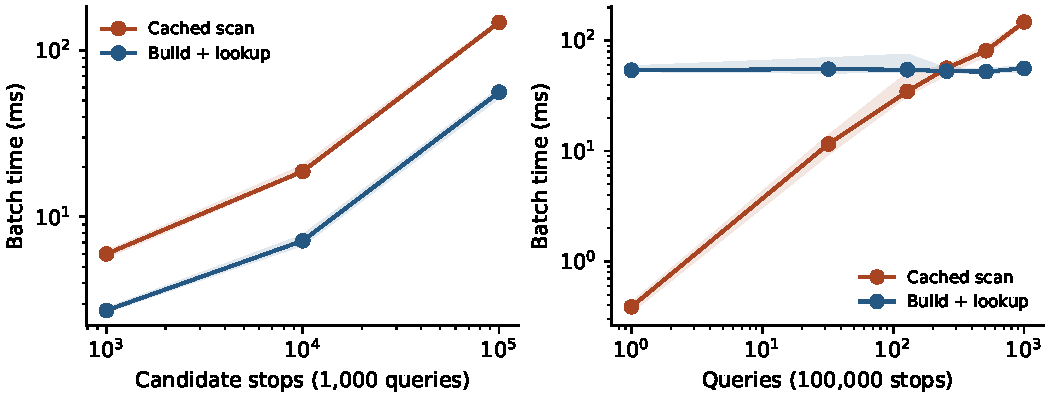
\includegraphics[width=\linewidth]{runtime.pdf}\\
\small Figure 2. Measured batch times on logarithmic axes. Points are medians
of five trials; shading spans the minimum and maximum. Lines join measured
workloads. Left: grow the list. Right: reuse the same list more often.
\end{center}

\paragraph{Interpretation.}
The two panels answer different planning questions. Increasing the number
of stops makes a scan more expensive for every cutoff. Increasing the number
of queries spreads the one-time sorting and prefix computation over more
decisions. The 100,000-stop lookup batch alone took 2.31 ms, but a planner
starting with coordinates also pays the build cost. That distinction explains
why the same implementation loses on a single query and wins on a long batch.

\paragraph{Scope and reproduction.}
The result concerns exactly one intermediate stop, a fixed list and Euclidean
travel length. Road travel times, moving stops and multiple transfers are
outside the experiment. The empirical baseline is an in-memory vectorized
scan. The minimum-distance observation supplies the scalar threshold, and
the sorted prefix minimum exploits its order. The probability law of the
stops plays no role in the proof.

\begingroup\raggedright
From the repository root, run \texttt{python -m routing\_note.experiment}
to regenerate \texttt{timings.csv}. Run \texttt{python -m routing\_note.figures}
to render both vector figures from the example and the recorded trials.
The timed index is in \texttt{triangle\_companion/one\_stop.py}. For the
shape-space formulation see Jonathan R. Landers, \textit{How large must a
triangle be to survive?}, in that companion folder.\par\endgroup
\end{document}
